

\tikzset{every picture/.style={line width=0.75pt}} %set default line width to 0.75pt        

\begin{tikzpicture}[x=0.75pt,y=0.75pt,yscale=-1,xscale=1]
%uncomment if require: \path (0,138); %set diagram left start at 0, and has height of 138

%Straight Lines [id:da8062637216156805] 
\draw[->]    (70,80) -- (270,80) ;
%Straight Lines [id:da31337861884224827] 
\draw[<-]    (70,110) -- (270,110) ;
%Straight Lines [id:da9857458477267009] 
\draw[->]    (310,70) -- (510,70) ;

% Text Node
\draw (2,3) node [anchor=north west][inner sep=0.75pt]   [align=left] {Alice};
% Text Node
\draw (2,23) node [anchor=north west][inner sep=0.75pt]   [align=left] {input: $\displaystyle a$};
% Text Node
\draw (170,76.6) node [anchor=south] [inner sep=0.75pt]    {$x_{\mathrm{a}}\leftarrow a+k_{0}$};
% Text Node
\draw (170,106.6) node [anchor=south] [inner sep=0.75pt]    {$x\leftarrow rx_{\mathrm{a}} -x_{\mathrm{b}}$};
% Text Node
\draw (-5,110.05) node [anchor=west] [inner sep=0.75pt]    {$x+k_{1}\overset{?}{=} 0$};
% Text Node
\draw (410,66.6) node [anchor=south] [inner sep=0.75pt]    {$r,\ \ \ x_{\mathrm{b}}\leftarrow r( b+k_{0}) +k_{1}$};
% Text Node
\draw (545,71.6) node [anchor=south] [inner sep=0.75pt]    {$r\overset{\mathrm{R}}{\leftarrow }\mathbb{Z}_{p}$};
% Text Node
\draw (290,3) node [anchor=north] [inner sep=0.75pt]   [align=left] {Server};
% Text Node
\draw (290,23) node [anchor=north] [inner sep=0.75pt]   [align=left] {Sam};
% Text Node
\draw (522,3) node [anchor=north west][inner sep=0.75pt]   [align=left] {Bob};
% Text Node
\draw (522,23) node [anchor=north west][inner sep=0.75pt]   [align=left] {input: $\displaystyle b$};


\end{tikzpicture}